\documentclass[12pt,a4paper,twoside,openright]{report}
% UPDATED BY MARCUS SCHAGERBERG, 2023
% CREATED BY DAVID FRISK, 2016

% BASIC SETTINGS
\usepackage{moreverb}								% List settings
\usepackage{textcomp}								% Fonts, symbols etc.
\usepackage{lmodern}								% Latin modern font
\usepackage{helvet}									% Enables font switching
\usepackage[T1]{fontenc}							% Output settings
\usepackage[english]{babel}							% Language settings
\usepackage[utf8]{inputenc}							% Input settings
\usepackage{amsmath}								% Mathematical expressions (American mathematical society)
\usepackage{amssymb}								% Mathematical symbols (American mathematical society)
\usepackage{graphicx}								% Figures
\usepackage{subfig}									% Enables subfigures
\numberwithin{equation}{chapter}					% Numbering order for equations
\numberwithin{figure}{chapter}						% Numbering order for figures
\numberwithin{table}{chapter}						% Numbering order for tables
\usepackage[outputdir=../]{minted}				    % Enables source code listings
\usepackage[top=3cm, bottom=3cm,
			inner=3cm, outer=3cm]{geometry}			% Page margin lengths			
\usepackage{eso-pic}								% Create cover page background
\newcommand{\backgroundpic}[3]{
	\put(#1,#2){
	\parbox[b][\paperheight]{\paperwidth}{
	\centering
	\includegraphics[width=\paperwidth,height=\paperheight,keepaspectratio]{#3}}}}
\usepackage{float} 									% Enables object position enforcement using [H]
\usepackage{datetime} %date formatting tools
\usepackage[title]{appendix} % For using \begin{appendices} instead of \appendix since that adds an extra section


% OPTIONAL SETTINGS (DELETE OR COMMENT TO SUPRESS)

% Caption settings (aligned left with bold name)
\usepackage[labelfont=bf, textfont=normal,
			justification=justified,
			singlelinecheck=false]{caption} 		

		  	
% Activate clickable links in table of contents  	
\usepackage{hyperref}								
\hypersetup{colorlinks, citecolor=black,
   		 	filecolor=black, linkcolor=black,
    		urlcolor=black}


% Define the number of section levels to be included in the t.o.c. and numbered	(3 is default)	
\setcounter{tocdepth}{5}							
\setcounter{secnumdepth}{5}	


% Chapter title settings
\usepackage{titlesec}		
\titleformat{\chapter}[display]
  {\Huge\bfseries\filcenter}
  {{\fontsize{50pt}{1em}\vspace{-4.2ex}\selectfont \textnormal{\thechapter}}}{1ex}{}[]


% Header and footer settings (Select TWOSIDE or ONESIDE layout below)
\usepackage{fancyhdr}								
\pagestyle{fancy}  
\renewcommand{\chaptermark}[1]{\markboth{\thechapter.\space#1}{}} 


% Select one-sided (1) or two-sided (2) page numbering
\def\layout{2}	% Choose 1 for one-sided or 2 for two-sided layout
% Conditional expression based on the layout choice
\ifnum\layout=2	% Two-sided
    \fancyhf{}			 						
	\fancyhead[LE,RO]{\nouppercase{ \leftmark}}
	\fancyfoot[LE,RO]{\thepage}
	\fancypagestyle{plain}{			% Redefine the plain page style
	\fancyhf{}
	\renewcommand{\headrulewidth}{0pt} 		
	\fancyfoot[LE,RO]{\thepage}}	
\else			% One-sided  	
  	\fancyhf{}					
	\fancyhead[C]{\nouppercase{ \leftmark}}
	\fancyfoot[C]{\thepage}
\fi


% Enable To-do notes
\usepackage[textsize=tiny]{todonotes}   % Include the option "disable" to hide all notes
\setlength{\marginparwidth}{2.5cm} 


% Supress warning from Texmaker about headheight
\setlength{\headheight}{15pt}		

\usepackage{modules/frontmatter/commands}

\usepackage{../preamble}
\usepackage{amsmath}
\usepackage{tikz}
\usepackage{standalone}
\usepackage{rotating}
\usepackage{tabularx}
\usepackage{multirow}
\usepackage{float}
\usepackage{adjustbox}
\usepackage{graphicx}
\usepackage{fancyhdr}
\usepackage{xcolor}
\usepackage{siunitx}

\usepackage{listings}
\lstdefinestyle{csharp}{
  language=[Sharp]C,
  frame=single,
  showspaces=false,
  showtabs=false,
  breaklines=true,
  showstringspaces=false,
  breakatwhitespace=true,
  escapeinside={(*@}{@*)},
  basicstyle=\ttfamily\small,
  keywordstyle=\color{blue},
  commentstyle=\color{green!40!black},
  stringstyle=\color{red!60!black}
}
\usepackage{caption}


% Add fancyhdr lines
\renewcommand{\headrulewidth}{0.5pt}
\renewcommand{\footrulewidth}{0pt}

% Title of the thesis
\newcommand{\oneLineTitle}{Simulating Traffic Flows}
\newcommand{\multiLineTitle}[1]{Simulating Traffic Flows and\\[#1]  Analysing Road Network Design}
\newcommand{\oneLineSubtitle}{Investigating the relationship between road network design and traffic congestion}


\begin{document}

% Roman numbering (starting with i (one)) until first main chapter
\pagenumbering{roman}

% Cover page, Title page and Imprint page
% UPDATED BY MARCUS SCHAGERBERG, 2023
% CREATED BY WOLFGANG AHRENDT, 2021
% BASED ON A MASTER THESIS TEMPLATE CREATED BY DAVID FRISK, 2016,
%        MODIFIED BY JAKOB JARMAR 2016 AND GUSTAV ÖRTENBERG 2019

% COVER PAGE
\begin{titlepage}
\newgeometry{top=3cm, bottom=3cm,
			left=2.25 cm, right=2.25cm}	% Temporarily change margins		
			
% Cover page background 
\AddToShipoutPicture*{\backgroundpic{-4}{56.7}{modules/frontmatter/frontpage_gu_eng_vec_m2.pdf}}
\addtolength{\voffset}{2cm}

% Cover picture (replace with your own or delete)		
\begin{figure}[H]
    \centering
    % Adjust vertical spacing here
    \vspace{1cm}
    %\includegraphics[width=0.9\linewidth]{figure/somepicture}
\end{figure}

% Cover text
\mbox{}
\vfill

% Set cover page font
\renewcommand{\familydefault}{\sfdefault} \normalfont 

\textbf{\Huge \multiLineTitle{0.2cm}} 
\\[0.5cm]

{\Large \oneLineSubtitle}\\[0.5cm]

%{\Large A Subtitle that can be Very Much Longer if Necessary}\\[0.5cm]

Bachelor's thesis in Computer science and engineering \setlength{\parskip}{1cm}

{\Large \MARTIN} \setlength{\parskip}{2.9cm}\\[1ex]
{\Large \FELIX} \setlength{\parskip}{2.9cm}\\[1ex]
{\Large \HANNES} \setlength{\parskip}{2.9cm}\\[1ex]
{\Large \MARCUS} \setlength{\parskip}{2.9cm}\\[1ex]
{\Large \JAKOB} \setlength{\parskip}{2.9cm}

Department of Computer Science and Engineering \\
\textsc{Chalmers University of Technology} \\
\textsc{University of Gothenburg} \\
Gothenburg, Sweden \the\year

\renewcommand{\familydefault}{\rmdefault} \normalfont % Reset standard font
\end{titlepage}


% BACK OF COVER PAGE (BLANK PAGE)
\newpage
\restoregeometry
\thispagestyle{empty}
\mbox{}


% TITLE PAGE
\newpage
\thispagestyle{empty}
\begin{center}
	\textsc{\large Bachelor's thesis \the\year}\\[4cm]		% Report number is currently not in use
	\textbf{\Large \multiLineTitle{0.2cm}} \\[1cm]
	{\large \oneLineSubtitle}\\[1cm]
	{\large \MARTIN}\\[1ex]
	{\large \FELIX}\\[1ex]
	{\large \HANNES}\\[1ex]
	{\large \MARCUS}\\[1ex]
	{\large \JAKOB}
	
	\vfill	
	% Logotype on titlepage	
	\begin{figure}[H]
    	\centering
    	% Remove the following line to remove the titlepage logotype
    	
\includegraphics[width=0.25\pdfpagewidth]{modules/frontmatter/ChGULogoHog.pdf}
	\end{figure}	\vspace{5mm}	
	
	Department of Computer Science and Engineering\\
	%\emph{Division of Division name}\\
	%Name of research group (if applicable)\\
	\textsc{Chalmers University of Technology} \\
	\textsc{University of Gothenburg} \\
	Gothenburg, Sweden \the\year \\
\end{center}

% IMPRINT PAGE (BACK OF TITLE PAGE)
\newpage
\thispagestyle{plain}
\vspace*{4.5cm}
\oneLineTitle\\
\oneLineSubtitle\\
\MARTINT{} \setlength{\parskip}{1cm}
\FELIXT{} \setlength{\parskip}{1cm}
\HANNEST{} \setlength{\parskip}{1cm}
\\
\MARCUST{} \setlength{\parskip}{1cm}
\JAKOBT{} \setlength{\parskip}{1cm}

\copyright ~ \MEMBERTILDELIST{} \the\year. \setlength{\parskip}{1cm}

Supervisor: \supervisor, \supervisordepartment\\
(if applicable) Advisor: Name, Company or Institute\\
Examiner: Name, Department \setlength{\parskip}{1cm}

Bachelor's Thesis \the\year\\	% Report number currently not in use 
Department of Computer Science and Engineering\\
%Division of Division name\\
%Name of research group (if applicable)\\
Chalmers University of Technology and University of Gothenburg\\
SE-412 96 Gothenburg\\
Telephone +46 31 772 1000 \setlength{\parskip}{0.5cm}

\vfill
% Caption for cover page figure if used, possibly with reference to further information in the report
Cover: Description of the picture on the cover page (if applicable)


Typeset in \LaTeX \\
%Printed by [Name of printing company]\\
Gothenburg, Sweden \the\year



% Abstract
\newpage
% UPDATED BY MARCUS SCHAGERBERG, 2023
% CREATED BY DAVID FRISK, 2016

%\oneLineTitle\\
%\oneLineSubtitle\\
%\MEMBERTILDELIST\\

%Department of Computer Science and Engineering\\
%Chalmers University of Technology and University of Gothenburg\setlength{\parskip}{0.5cm}

% Supress header
\thispagestyle{plain} 
\setlength{\parskip}{0pt plus 1.0pt}
% WRITTEN BY MARTIN BLOM, 2023
\section*{Abstract}
    Tools for simulating traffic are important for transportation planning and to be able to analyse how road network changes will affect the traffic flows. This project aims to develop such a tool, with the distinction from existing tools that it should be intuitive to use and have a high accessibility for users. This thesis describes the development process and the methods used when creating the tool. It also dives into the different features it has and how they contribute to creating a realistic traffic simulator. From the user tests of the tool, it was found that it was intuitive and easy to use, but lacked in feature density and simulation tools when compared to existing tools.


    With the rise of large and densely populated cities, increased vehicular traffic is becoming more usual and with it comes an expected increase in traffic delays. We are all affected by this in one way or another, be it by personal transportation, resource shipping or any other situation. Moreover, traffic delays cost companies and governments large amounts of money and resources as well as increased emissions with reshipping or engines idling. The aim of this bachelor thesis is to combat these problems by developing a traffic simulation tool, used to analyse road network performance in the hopes to foresee probable issues and help with finding solutions.
    \\\\
    The simulation tool will be developed within Unity using the programming language C\# and will allow users to input traffic parameters such as traffic volume, vehicle types, and road infrastructure details. One of the main goals is for the tool to be intuitive and easy to operate for users. Therefore, a lot of weight is put into developing a user-friendly presentation of statistics. To help with achieving this, user-testing will be carried out and any interfaces in need of change will be tweaked and refined according to the feedback. Moreover, the tool will offer real-time visualization of the simulation, which is not often found in similar tools. Finally the results will be visualized using graphs and charts to provide a comprehensive analysis of traffic flow, including aspects such as traffic density, average speed, and queue length.
    \\\\
    The finished product will not be a fully realistic simulator, but a robust base software with good potential to be built upon and improved. To promote this, the whole project will be made open source making it accessible to anyone wanting to use or further develop it.

\newpage
% WRITTEN BY MARTIN BLOM, 2023
\section*{Sammandrag}
    Med en ökning av städer med hög befolkningstäthet blir ökad fordonstrafik vanligare och med det följer förväntade ökningar av trafikstörningar. Vi påverkas alla av detta på ett eller annat sätt, antingen genom persontransport, resursleveranser eller i andra situationer. Dessutom kostar trafikstörningar företag och regeringar stora mängder pengar och resurser, samt leder till ökade utsläpp genom omleveranser eller tomgångskörning av motorer. Syftet med denna kandidatuppsats är att bekämpa dessa problem genom att utveckla ett trafiksimuleringsverktyg som används för att analysera prestandan i vägnätet i förhoppningen om att förutse potentiella problem och hjälpa till att hitta lösningar.
    \\\\
    Simuleringsverktyget kommer att utvecklas inom Unity med programmeringsspråket C\# och tillåta användare att mata in trafikparametrar så som trafikvolym, fordonstyper och väginfrastrukturinformation. Ett av huvudmålen är att verktyget ska vara intuitivt och lätt att använda. Därför läggs stor vikt vid att utveckla en användarvänlig presentation av statistik. För att hjälpa till med detta kommer användartester att utföras och alla gränssnitt som behöver ändras kommer att justeras och förfinas enligt feedbacken. Dessutom kommer verktyget att erbjuda realtidsvisualisering av simuleringen, vilket ofta inte finns i liknande verktyg. Slutligen kommer resultaten att visualiseras med grafer och diagram för att ge en omfattande analys av trafikflödet, inklusive aspekter så som trafiktäthet, genomsnittlig hastighet och kölängd. 
    \\\\
    Den färdiga produkten kommer inte att vara en fullständigt realistisk simulator, utan en robust grundprogramvara med god potential att förbättras och byggas vidare på. För att främja detta kommer hela projektet att göras till öppen källkod så att det är tillgängligt för alla som vill använda eller vidareutveckla det.

% KEYWORDS (MAXIMUM 10 WORDS)
\vfill
Keywords: traffic, simulation, flow, emissions, vehicles, driving,

% Create empty back of side
\newpage
\thispagestyle{empty}
\mbox{}

% Ackowledgements
\newpage
% UPDATED BY MARCUS SCHAGERBERG, 2023
% CREATED BY DAVID FRISK, 2016
% Supress header
\thispagestyle{plain}
\section*{Acknowledgements}
    We would like to express our gratitude towards our supervisor, Natasha Bianca Mangan, who provided great guidance through our development process. With her experience, she helped us with specialised advice in the development software used in the project. In addition, her feedback for this report was invaluable.

    Special thanks go to our testers, without whom our tool would not have become as intuitive to use or accessible for users without extensive experience in transportation planning. With their feedback we were able to improve the user experience.

\vspace{1.5cm}
\hfill
\membertildelist{} Gothenburg, \monthname \space \the\year

% Create empty back of side
\newpage

% Table of contents
\newpage
\tableofcontents

%% Other frontmatter %%

% List of figures (add to table of contents)
\cleardoublepage
\addcontentsline{toc}{chapter}{\listfigurename} 
\listoffigures

% List of tables (add to table of contents)
\cleardoublepage
\addcontentsline{toc}{chapter}{\listtablename}  
\listoftables

% Glossary
\newpage
\section*{Glossary}
    \noindent
\label{itm:a*}\textbf{A*}: A popular graph traversal and path searching algorithm due to its completeness and optimal efficiency. A* is used to find the shortest possible path from one node to another.

\noindent
\label{itm:agent}\textbf{Agent}: Autonomous entities that inhabits an environment and act based on predefined rules.

\noindent
\label{itm:abm}\textbf{Agent Based Model (ABM)}: A computer simulation model in which agents interact with each other and their environment to produce emergent behavior. 

\noindent
\label{itm:csharp}\textbf{C\#}: C\# is a programming language developed by Microsoft that runs on the platform .NET Framework. C\# is pronounced as "C sharp" and belongs to the programming language family of C.

\noindent
\label{itm:c++}\textbf{C++}: One of the most popular general purpose programming languages. C++ is pronounced as "C plus plus" and belongs to the programming language family of C, with the major distinction from C that C++ is an object oriented language.

\noindent
\label{itm:data-structure}\textbf{Data Structure}: A way of organizing and storing data in a computer so that i can be accessed, manipulated, and modified efficiently. Some common examples are arrays, stacks, and linked lists. 

\noindent
\label{itm:fps}\textbf{FPS}: Frames Per Second, is a unit used for measuring software performance, usually in games. It is the number of images displayed per second. A higher FPS gives a smoother experience.

\noindent
\label{itm:information-visualization}\textbf{Information Visualization}: Field that focuses on creating meaningful and easy to to interpret graphical representations of data.

\noindent
\label{itm:monobehaviour}\textbf{MonoBehaviour}: Base class for Unity scripts. Provides access to event functions such as Start(), Update(), and so on.

\noindent
\label{itm:open-street-map}\textbf{OSM}: OpenStreetMap is an open source database containing map data.

\noindent
\label{itm:pooling}\textbf{Pooling}: A technique used in programming to improve performance by reusing objects instead of creating new ones. 

\noindent
\label{itm:prefab}\textbf{Prefab}: A reusable object in Unity that stores a configuration and can be used as a template for creating assets.

\noindent
\label{itm:repository}\textbf{Repository}: A repository acts as a container that stores a projects files and their individual revision history. 

\noindent
\label{itm:scrum}\textbf{Scrum}: The scrum agile project management framework provides structure and management of work and is popular among software development teams.

\noindent 
\label{itm:scrum-boards}\textbf{Scrum-boards}: A bulletin board that keeps track of a backlog, the current sprint, and completed stories.

\noindent
\label{itm:story}\textbf{Story}: In the scrum framework, a story is essentially a set of tasks that will result in a new or updated desired functionality/product.  

\noindent
\label{itm:ui}\textbf{UI}: UI, or User Interface, is the connection between humans and computers. It determines how the user interacts with the program.

\noindent
\label{itm:unity}\textbf{Unity}: Cross-platform game engine.

\noindent
\label{itm:unity-asset}\textbf{Unity Asset}: A file  containing reusable content that can be imported into Unity projects. Can be accessed through Unity's official platform or imported via third-party repositories. 

\noindent
\label{itm:user-testing}\textbf{User Testing}: A method of testing and evaluating a product by observing and gathering data from real users. 

\noindent
\label{itm:ux}\textbf{UX}: UX, or User Experience, refers to the overall experience of the actual user of a product. The goal of good UX design is to create intuitive and enjoyable products.

%\noindent
%\label{itm:wire-frame}\textbf{Wire Frames}: Wire Frames depict how the UI layout will appear during different stages of the program. 


\thispagestyle{plain}

%% Start of main document %%
\cleardoublepage
\setcounter{page}{1}
% Arabic numbering starting from 1 (one)
\pagenumbering{arabic}
% Set the vertical distance between paragraphs
\setlength{\parskip}{10pt}

% Introduction
\chapter{Introduction}
    % UPDATED BY MARCUS SCHAGERBERG, 2023
% CREATED BY DAVID FRISK, 2016

Make sure you have read the abstract of this template.
This chapter presents the section levels that can be used in the template. 

\section{Section levels}
The following table presents an overview of the section levels that are used in this document. The number of levels that are numbered and included in the table of contents is set in the settings file \texttt{settings.tex}. The levels are shown in Section \ref{Section_ref}.

\begin{table}[H]
\centering
\begin{tabular}{ll} \hline\hline
Name & Command\\ \hline
Chapter & \textbackslash\texttt{chapter\{\emph{Chapter name}\}}\\
Section & \textbackslash\texttt{section\{\emph{Section name}\}}\\
Subsection & \textbackslash\texttt{subsection\{\emph{Subsection name}\}}\\
%Paragraph & \textbackslash\texttt{paragraph\{\emph{Paragraph name}\}}\\
%Subparagraph & \textbackslash\texttt{paragraph\{\emph{Subparagraph name}\}}\\ \hline\hline
\end{tabular}
\end{table}

\section{Related Work} \label{Section_ref}
\subsection{Microscopic Traffic Simulations}
There exists a plethora of different available tools for traffic simulation, which are in turn built upon different underlying models. In Nguyen’s widely cited paper, he classifies the currently available simulations according to the following four categories with regards to their granularity of model: Macroscopic, Microscopic, Mesoscopic, and Nanoscopic. These tools allow researchers to answer complex questions and evaluate different scenarios in both real-time observations and through post-simulation data analysis. \\

Agent-based traffic models position themselves within the Microscopic category and allows for a highly realistic representation of traffic flow, where emergent behaviors such as congestion and bottleneck formation can occur due to the natural occurring interplay of the autonomous agents within the simulation. \\

Simulation of Urban MObility (SUMO) is a widely used and open source microscopic traffic simulation which includes functionality that allows the user to model different transportation agents such as cars, buses, bicycles, and pedestrians in both an urban environment. The simulation is by default deterministic but stochastic processes can be introduced in various ways. \\

The software offers various tools creating networks and editing these through a map editor which can also import and export network data from external sources. In addition to this, SUMO provides the user with features for visualizing the obtained data and analyzing it through various reports and plots. Users can also customize SUMO to accommodate their specific need through the application programming interface (API) and integrate the simulation with other software. \\ 


% Theory
\chapter{Theory}
    % UPDATED BY MARCUS SCHAGERBERG, 2023
% CREATED BY WOLFGANG AHRENDT, 2021

% WRITTEN BY FELIX JÖNSSON, 2023
This section lays the theoretical foundation for the essential concepts that underpin the implementation of our agent-based traffic model in Unity. It covers a variety of topics, including specific mathematical functions, code design principles, pathfinding algorithms, and the theoretical aspects of software development project management frameworks. By establishing a solid understanding of these core concepts, readers will be better prepared to grasp the intricacies of the traffic simulation presented later in this thesis.

% WRITTEN BY FELIX JÖNSSON, 2023
\section{Unity}

A game engine is a software framework designed to facilitate the creation of video games by providing the most commonly needed functionalities. These include complex tasks such as physics calculations, animation, rendering, and artificial intelligence. The advantage of using a pre-existing game engine is that it allows developers to focus on the unique aspects of their game and accelerates the development pipeline, as they do not have to code these complex systems from scratch.

Unity is a game engine initially released for Mac OS X in 2005 at the Apple Worldwide Developers Conference\cite{macworld2005}. The CEO of the company has said that the mission was to democratize game development, making it widely accessible to a broad audience\cite{polygon2014}. By 2022, the company had secured a significant market share of 38\%, signifying its wide acceptance and popularity within the industry\cite{slashdata2022}.

Unity can be used to produce both 2D and 3D environments, and it offers native support for a wide variety of platforms and operating systems. Although there is a wealth of underlying theory supporting the engine, of which the most prominent is considered to be the Component-Based Object Model. Development in Unity is centered around so-called GameObjects, which serve as the base class for all entities in Unity scenes. These GameObjects can then receive different components, which can take the form of a wide range of things, such as scripts, textures, cameras, and so on. This pattern allows for a flexible and modular development approach, as many GameObjects can reuse the same component while customizing each component parameter to their specific requirements.

Another central underlying theory is that of Event-Driven Programming and the implementation of a so-called game loop\cite{gameprogrammingpatterns2023}. By using an event-centric communication method for many of its native systems such as input handling and collision detection, components such as scripts can define methods that hook onto the event architecture. These can then respond to specific events such as "OnCollisionEnter", which is called when a collision occurs\cite{unityManualExecutionOrder2023}\cite{unityManualEventFunctions2023}. This Event-Driven approach works in symbiosis with the theory of a game loop. A game loop is a ubiquitous architecture technique used within the game engine sphere. The basic concept is that an update event occurs each frame, also called a tick, where all GameObjects and their components have the opportunity to react and update themselves according to the current state of their environment. Since these updates occur with high frequency, often many times per second, this allows the game to simulate real-time behavior.



\newcommand{\timeconstraint}{, \quad 0 \le t \le 1}
\newcommand{\lerp}{\rightarrow}
\newcommand{\p}[1]{P\textsubscript{#1}}

% Marcus Schagerberg
\section{Bézier curves}
    A Bézier curve is a parametric curve between two points, that curves according to a set of intermediate points. The points are called control points, where the first and last point are the endpoints of the curve. A linear Bézier curve only has two points, which means that it is a line between the points. It is defined by the following function:

    $$
        P(t) = (1-t)^2P_0 + 2t(1-t)P_1 + t^2P_2 \timeconstraint
    $$

    The parameter $t$ is the ratio along the line, with $t = 0$ and $t = 1$ marking the endpoints. This is what is known as linear interpolation in mathematics. A linear Bézier curve is therefore simply a linear interpolation between the points $P_0$ and $P_1$. Let's define this as $P_0 \lerp P_1$. The quadratic Bézier curve consists of two linear interpolations:
    
    $$ A) \quad P_0 \lerp P_1$$
    $$ B) \quad P_1 \lerp P_2 $$
    
    It is then defined as the linear interpolation between these points, i.e $ A \lerp B $. All linear interpolations in this case depend on the same $t$, which is what creates the curvature of the Bézier curves.

    Since a quadratic Bézier curve has three points, it will have two endpoints as well as an additonal control point between them. By moving the control point, the shape of the Bézier curve can be altered. This is presented with the following examples, the first three of which have static endpoints demonstrating how the middle control point can be used to form the curve. The final example eludes to the fact that the control points can be placed anywhere without the requirement of any order.

    \begin{figure}[H]
        \begin{tabular}{cc}
            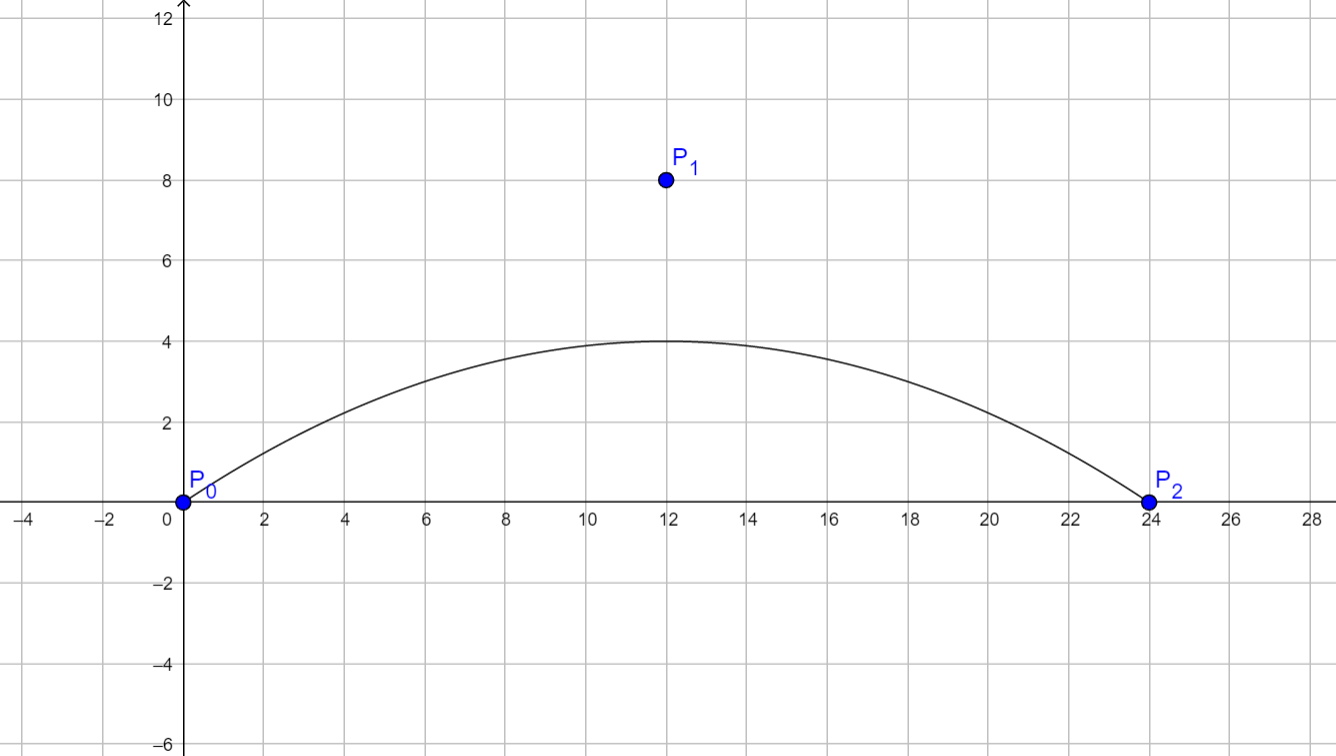
\includegraphics[width=0.5\linewidth]{figures/theory/bezier_curves/quadratic1.png} & 
            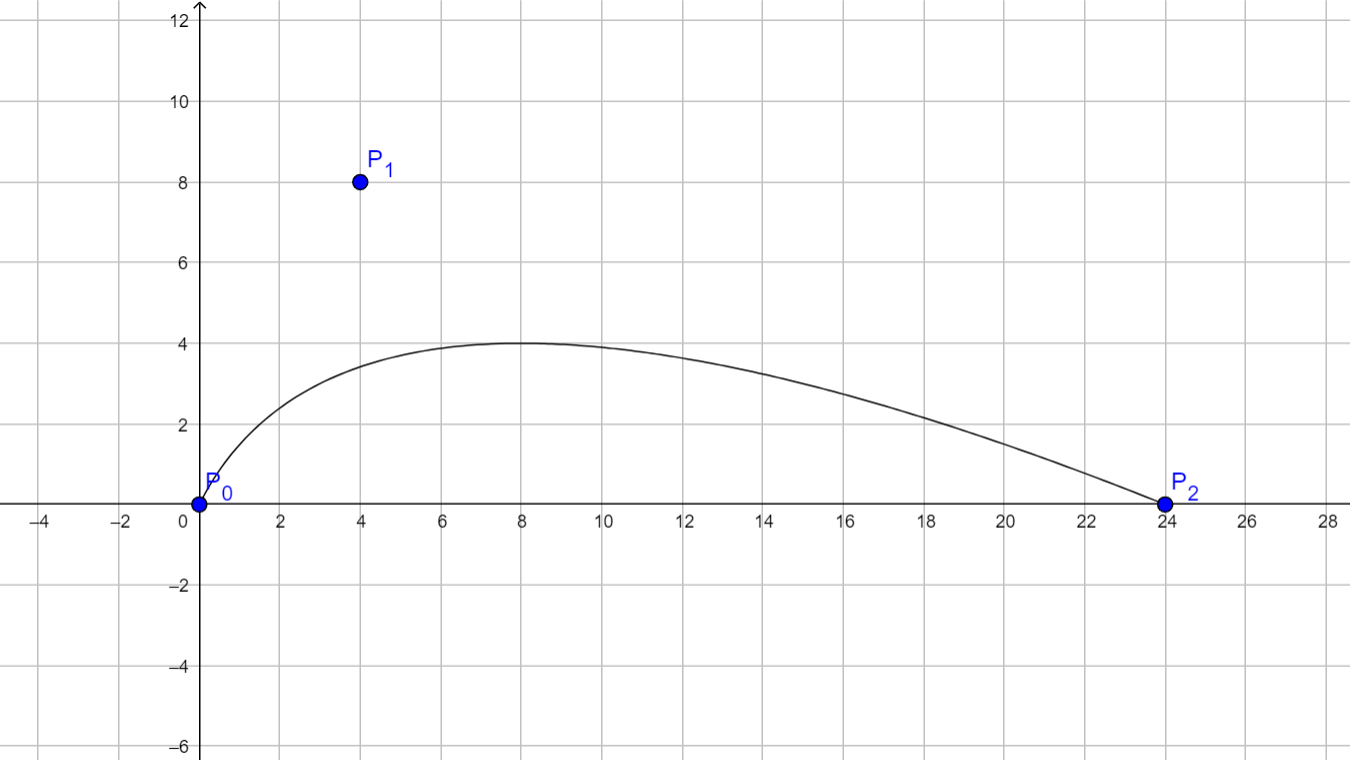
\includegraphics[width=0.5\linewidth]{figures/theory/bezier_curves/quadratic2.png} \\
            
            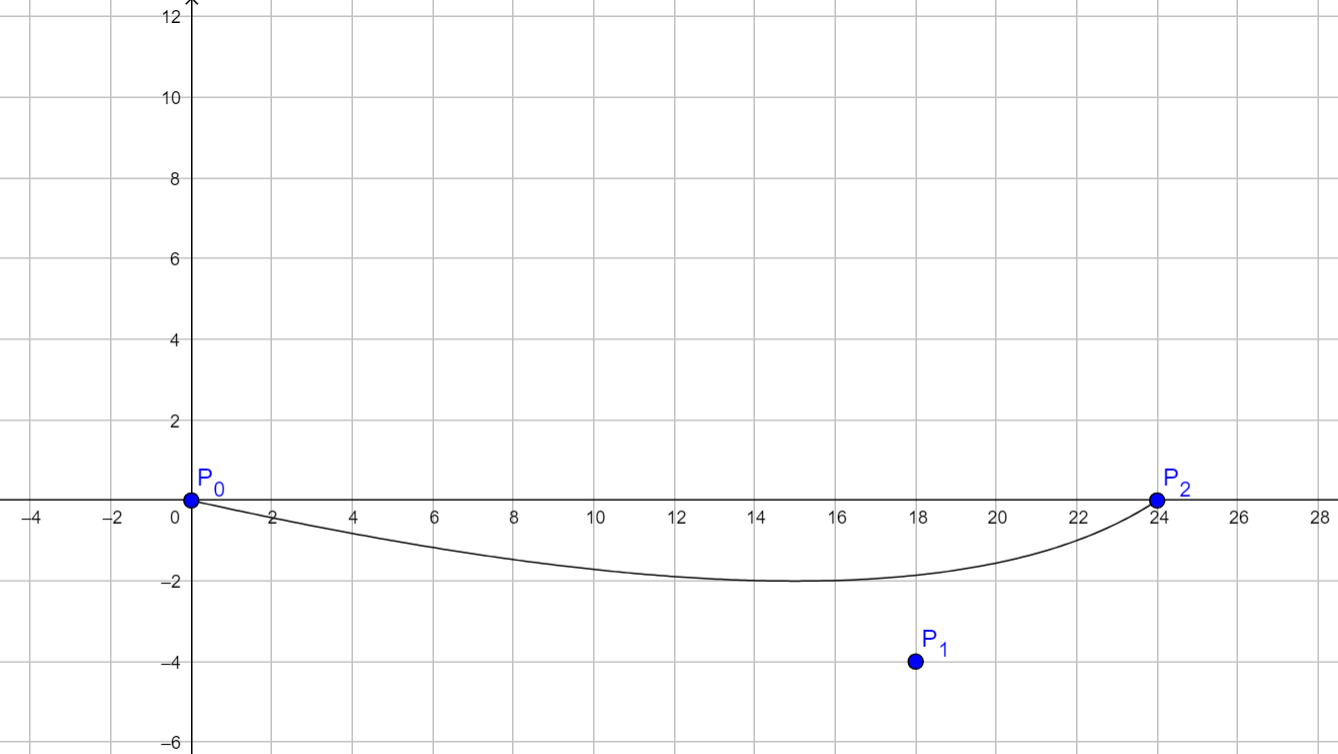
\includegraphics[width=0.5\linewidth]{figures/theory/bezier_curves/quadratic3.png} & 
            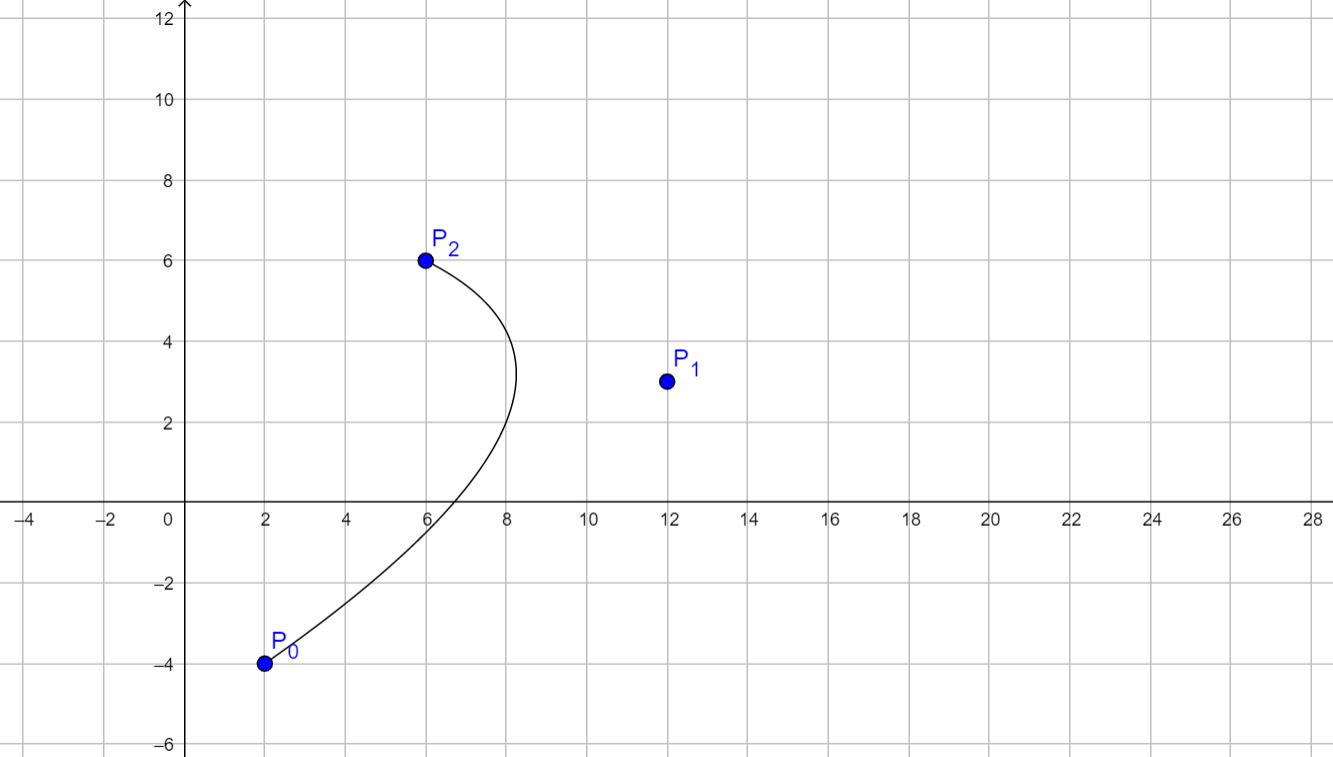
\includegraphics[width=0.5\linewidth]{figures/theory/bezier_curves/quadratic4.png}
        \end{tabular}
        \caption{Four examples of quadratic Bézier curves}
    \end{figure}

    
    
    % Hannes Kaulio and Marcus Schagerberg
    \subsection{Cubic Bézier Curve}
        A cubic Bézier curve expands on the quadratic curve in the same fashion as the quadratic expanded on the linear Bézier curve, adding another layer of linear interpolations. A cubic Bézier curve has four control points, two of which are endpoints.
        
        \inlineimage{figures/theory/bezier_curves/bezier_curve.png}{Cubic Bézier curve with control points \p{0}, \p{1}, \p{2} and \p{3}}{0.5}
    
        The cubic Bézier curve can be defined by the formula\cite{Cubic-Bézier-Curves}: 
        $$
            P(t) = (1-t)^3P_0 + 3t(1 - t)^2P_1 + 3t^2(1 - t)P_2 + t^3P_3 \timeconstraint
        $$
        Properties of the Cubic Bézier curve relevant to this paper are the following:
        \begin{enumerate}
            \item The endpoints \p{0} and \p{3} lay on the curve
            \item The curve is continuous, infinitely differentiable, and the second derivatives are continuous.
            \item The tangent line to the curve at the point \p{0} is the line \p{0}\p{1}. The tangent to the
        curve at the point \p{3} is the line \p{2}\p{3}.
            \item Both \p{1} and \p{2} lay on the curve only if the curve is linear.
            \item A Bézier curve is contained within the convex hull of the control points. For the application in Unity, this means that a Bézier curve is completely contained within the bounding box created by its control points.
        \end{enumerate}

    % Marcus Schagerberg
    \subsection{De Casteljau's algorithm}
        In 1959 the french mathematician Paul de Casteljau constructed an algorithm for dividing a Bézier curve into two. The union of these Bézier segments is equivalent to the original curve.
    
    % Marcus Schagerberg
    \subsection{Bézier Clipping}
        Finding the intersection points between two Bézier paths is not as straight forward as for something like two lines. To solve this, an algorithm called Bézier clipping explained in \cite{bezier-clipping} can be used. It utilises the convex hull property of Bézier curves - and therefore Bézier paths - as well as de Casteljau's algorithm for splitting curves. An implementation for finding all intersection points between two Bézier paths using Bézier clipping is outlined below.

        \vspace{1cm}
        \begin{algorithmic}
            \State $intersections \gets$ Empty list
            \State $epsilon \gets$ A value >0 small enough for the desired accuracy
            \Procedure{FindBezierPathIntersections}{$A, B$}
                \If{$A.BoundingBox$ does not intersect $B.BoundingBox$}
                    \State \Return
                \EndIf

                \If{$A.BoundingBox.Size$ + $B.BoundingBox.Size < epsilon$}
                    \State $intersections \gets$ Midpoint between A and B
                    \State \Return
                \EndIf

                \State $A_1, A_2 \gets SplitWithDeCasteljau(A, 0.5)$
                \State $B_1, B_2 \gets SplitWithDeCasteljau(B, 0.5)$

                \State $FindBezierPathIntersections(A_1, B_1)$
                \State $FindBezierPathIntersections(A_1, B_2)$
                \State $FindBezierPathIntersections(A_2, B_1)$
                \State $FindBezierPathIntersections(A_2, B_2)$
            \EndProcedure
        \end{algorithmic}
        \vspace{1cm}

        Worth noting is the $Midpoint$, which is one of many possible approximations of the intersection point. For a small enough $epsilon$, the approximation used is trivial as the segments approaches points as $epsilon$ approaches 0.

    % Hannes Kaulio and Marcus Schagerberg
    \subsection{Composite Bézier curve}
        A composite Bézier curve is a spline made out of Bézier curves. The series of Bézier curves are joined together end to end with the start point of one curve coinciding with the end point of the other curve. This is used in the projects as it allows for chaining of cubic Bézier path segments creating a spline. 

% Hannes Kaulio + Felix 
% Hannes Kaulio + Felix 
\section{A* Algorithm}
    A* is an algorithm widely used for pathfinding and graph traversal. Peter Hart, Nils Nilsson, and Bertram Raphael first presented the algorithm in 1968 as part of a project focused on constructing a mobile robot capable of autonomously devising its actions\cite{hart1968formal}. It is classified as an informed search algorithm since it greedily explores the pathfinding environment by taking into account both the cost of the path from the starting node to the one that is currently being explored. A heuristic function that estimates the distance between the currently explored node and the goal node is also used\cite{russell2016artificial}. Given a start and end node in a weighted graph, the algorithm will find the shortest path between the nodes. Together, these two form an estimate function of the best path towards the goal. A* is complete under the precondition that the search space is finite, and the branching factor is also finite, which guarantees that if a path exists, it will be found. Furthermore, if some additional conditions are fulfilled with regards to the heuristic function, A* can be guaranteed to return an optimal path. For this to be the case, the heuristic function needs to be admissible or consistent, since a consistent function is also, by definition, admissible\cite{dechter1985generalized}.

    In the project, we aim to implement the A* algorithm to find the shortest path on a graph consisting of nodes representing intersections, road ends, and points of interest (POIs). Here, POIs primarily serve as target destinations for our agents and may include parking lots, fuel stations and other relevant locations. By implementing the A* algorithm, we can develop dynamic heuristic functions that adapt to real-time events such as traffic accidents or road closures. This adaptability will lead to a more responsive system, ultimately improving the overall performance of the traffic simulation. 
    
    In order to implement the A* algorithm, an open and closed set of nodes are utilized, as well as a few essential variables and functions. These are the key elements used in the algorithm:

    \begin{itemize}
        \item Start node $s$: The initial position from which the search begins.
        \item Current node $n$: The node being evaluated during the search process.
        \item Target set $T$: Contains one or more goal nodes that the algorithm is trying to reach.
        \item Total estimated cost function $f(n)$: The sum of the cost from the start node to node $n$ (denoted by $g(n)$) and the heuristic estimate of the cost from the node $n$ to the target node (denoted by $h(n)$).
    \end{itemize}

    With these definitions in place, the A* algorithm can be described with the following procedure:

    \begin{enumerate}
        \item Label the start node $s$ as "open" and compute $f(s)$.
        \item Choose the open node $n$ with the smallest $f(s)$ value. In the case of a tie, the node is chosen randomly, but always prioritizes nodes in the target set $T$.
        \item If $n$ is in $T$, label $n$ as "closed" and conclude the algorithm.
        \item Otherwise, mark $n$ as closed and generate all adjacent nodes by exploring the neighboring nodes that can be reached from $n$ in the graph. Compute $f$ for each adjacent node of $n$ and label each adjacent node not already marked closed as "open". If a closed node $n_i$ is an adjacent node of $n$ and its current $f(n_{i})$ is smaller than its previous $f$ value when it was marked closed, relabel it as "open". Return to Step 2.
    \end{enumerate}

% Marcus Schagerberg
\section{Procedural mesh generation}
    All physical objects in Unity have an associated mesh, i.e. their surfaces. A cube for example can be thought of as having a mesh consisting of 6 different surfaces. In computer graphics, a triangle mesh is a type of mesh where the surfaces are created through a set of points, called vertices. These vertices are then joined together by a set of triangles. Going back to the cube example, a cube in its simplest form would have 12 triangles and 8 vertices. The eight vertices are at the corners of the cube. Each face of the cube has the shape of a square, which can be created with two triangles, hence double the amount of triangles as square faces.

\section{Scrum and Agile Software Development}
    Agile Software Development is a software development framework which emphasizes vertical development cycles, where software should be delivered frequently in atomic slices to enable quick feedback and high flexibility with regards to how the product develops. When developing complex products, and especially when the development team has not worked on anything similar to the current developed product, implementing an agile framework can be particularly important. Since features are delivered in small complete chunks, it minimizes the investment risk compared to a more horizontal feature development. 

% Felix 
\section{Agent Based Modeling}
    Agent-Based Modeling (ABM) is a computational modeling approach that facilitates the analysis and simulation of complex systems by depicting a system's individual elements (agents) and their interactions\cite{railsback2019agent}. This method enables researchers to investigate how the combined behavior of a system emerges from the attributes and actions of its individual components. In contrast to conventional models, which typically depend on mathematical tractability and differential equations for portraying behavior from a macroscopic viewpoint, ABMs face fewer restrictions and can encompass more aspects of real-world systems\cite{bonabeau2002agent}. As a result, these models can simulate intricate scenarios without relying on equally complex mathematics. It achieves this with satisfactory, and sometimes, even more precise outcomes compared to models that overlook the individual behaviors ABMs are capable of representing. It should be noted, though, that ABMs can also integrate more sophisticated mathematics and techniques, like neural networks or advanced learning approaches, to more accurately depict the complexities and dynamics of individual agents within the system.

\subsection{Key features}
    ABMs consist of individual agents that interact with each other and their environment. Agents can represent various entities such as organisms, humans, businesses, and so on. These agents are characterised by their uniqueness, local interactions, and autonomy. They can have different attributes such as size, location, and resource reserves, and they interact with their neighbors in a specific "space", such as a geographic area or a network\cite{railsback2019agent}. The mentioned space is typically relatively small in the scope of the total simulation space. Agents act independently and pursue their own objectives, adapting their behavior according to their current state, the state of other agents, and their environment.

\subsection{Emergence and across-level modeling}
    ABMs are particularly useful for studying emergent system behaviors that arise from the interactions and responses of individual components to each other and their environment. This allows researchers to explore how a system's dynamics are linked to the characteristics and behaviors of its individual components. Due to this, ABMs are considered across-level models because they focus on the interactions between the system level and the individual agent level\cite{railsback2019agent}. In these across-level models, the agents' behaviors and decision-making processes are modeled explicitly by the researchers, while the emergent properties of the system as a whole stem from these micro-level interactions that occur at run-time.

    Across-level models allow for a more nuanced understanding of complex systems, as they enable researchers to bridge the gap between micro-level interactions and macro-level outcomes. By capturing the heterogeneity of agents and their responses to their environment, across-level models can shed light on the mechanisms that drive system-level behavior, facilitating the identification of key feedback loops and dependencies within the system.

    Additionally, the models enable researchers to investigate the impact of various factors at both the individual and system levels, such as how changes in individual behaviors or environmental conditions may affect the overall system dynamics. This approach allows for a more thorough exploration of the robustness and adaptability of the system, providing valuable insights for policy development and system management.

\subsection{Advantages and applications}
    ABMs can address complex, multilevel problems that are too difficult to tackle with traditional models. Predator-prey dynamics serve as a classic example of a system traditionally modeled using differential equations and advanced calculus. However, these systems can also benefit from being modeled by an ABM\cite{railsback2020pred-prey}. By employing ABMs to study predator-prey interactions, researchers can gain deeper insights into the adaptive behaviors and decision-making processes of individual organisms. ABMs allow for the representation of heterogeneous agents and the examination of emergent properties arising from their interactions, which can be particularly valuable in understanding the complexities of real-world systems. Applying ABMs can bridge the gap between theoretical and empirical research, highlighting gaps in our knowledge of individual behaviors, and contribute to refining existing theories.

    Although the method appears straightforward to apply, researchers argue that this can create a false impression that the underlying concepts are just as simple to grasp. While ABM might seem technically uncomplicated, it possesses considerable conceptual depth, which frequently results in incorrect utilisation.

\section{Design Patterns}
    In software engineering, design patterns are common solutions for recurring problems encountered when building complex software. A design pattern can be described as a tried and tested blueprint based on well-known object-oriented principles, such as the SOLID\footnote{SOLID is an acronym that represents five important design principles for object-oriented programming. These are: Single Responsibility Principle, Open/Closed Principle, Liskov Substitution Principle, Interface Segregation Principle, and Dependency Inversion Principle. The purpose of these principles is to improve maintainability, readability, and extensibility.} principles that can be applied in many different contexts to solve various problems.

    Christopher Alexander initially introduced the idea of patterns in his book, "A Pattern Language: Towns, Buildings, Construction." In this work, he presented a "vocabulary" for designing urban landscapes. The building blocks of this vocabulary consist of patterns that address various aspects of urban design, such as the height of windows, the number of floors in a structure, the size of green spaces within a community, and other similar elements.

    This concept was later adapted by the "Gang of Four" (Erich Gamma, Richard Helm, Ralph Johnson, and John Vlissides) and translated to the domain of software engineering in their seminal book "Design Patterns: Elements of Reusable Object-Oriented Software," which was published in 1994. This book offers a catalog of 23 reusable design patterns for object-oriented programming that are based on industry experience and observations from the authors.

    Today, many design patterns have been integrated into programming languages themselves and are therefore taken for granted by users. For example, the Visitor pattern is a behavioral design pattern that allows you to separate the algorithm from the object structure it is supposed to operate on. One concrete realization of the Visitor pattern's integration into a modern programming framework can be found in the ubiquitous for-each loop. The for-each loop allows for iteration over a collection of elements without the need for an explicit counter index, effectively separating the algorithm responsible for the iteration from the underlying data structure.

    \begin{figure}[H]
        \begin{lstlisting}[style=csharp]
List<int> numbers = new List<int> { 1, 2, 3, 4, 5 };

for (int i = 0; i < numbers.Count; i++)
{
    Console.WriteLine(numbers[i] * 2);
}
        \end{lstlisting}
        \caption{For-loop}
          \label{fig:for-loop-example}
    \end{figure}


    \begin{figure}[H]
        \begin{lstlisting}[style=csharp]
static void DoubleAndLog(int number)
{
    Console.WriteLine(number * 2);
}

List<int> numbers = new List<int> { 1, 2, 3, 4, 5 };
numbers.ForEach(DoubleAndLog);
        \end{lstlisting}
        \caption{For-each loop implementing Visitor pattern}
          \label{fig:visitor-pattern-example}
    \end{figure}

\subsection{The Observer Pattern}
    One of the first design patterns introduced in the aforementioned book by the “Gang of Four”, the Observer pattern is a behavioral pattern that addresses several different key problems in object-oriented programming. It is implemented by creating two separate interfaces: the publisher who is responsible for publishing events of interest for the rest of the system, and subscribers who are interested in knowing when the publisher has published such an event. Implementing these interfaces allows the system to achieve loose coupling, as the publisher and subscribers can evolve independently, promoting a maintainable and adaptable system. Developers can easily introduce new subscribers with minimal modifications. Furthermore, the pattern facilitates dynamic relationships between scripts that can change at runtime by having the subscribers unsubscribe from the publisher. This, accompanied by the publisher's event broadcasting ability, ensures that the entire system remains in a consistent and traceable state. 

    \begin{figure}[H]
      \centering
      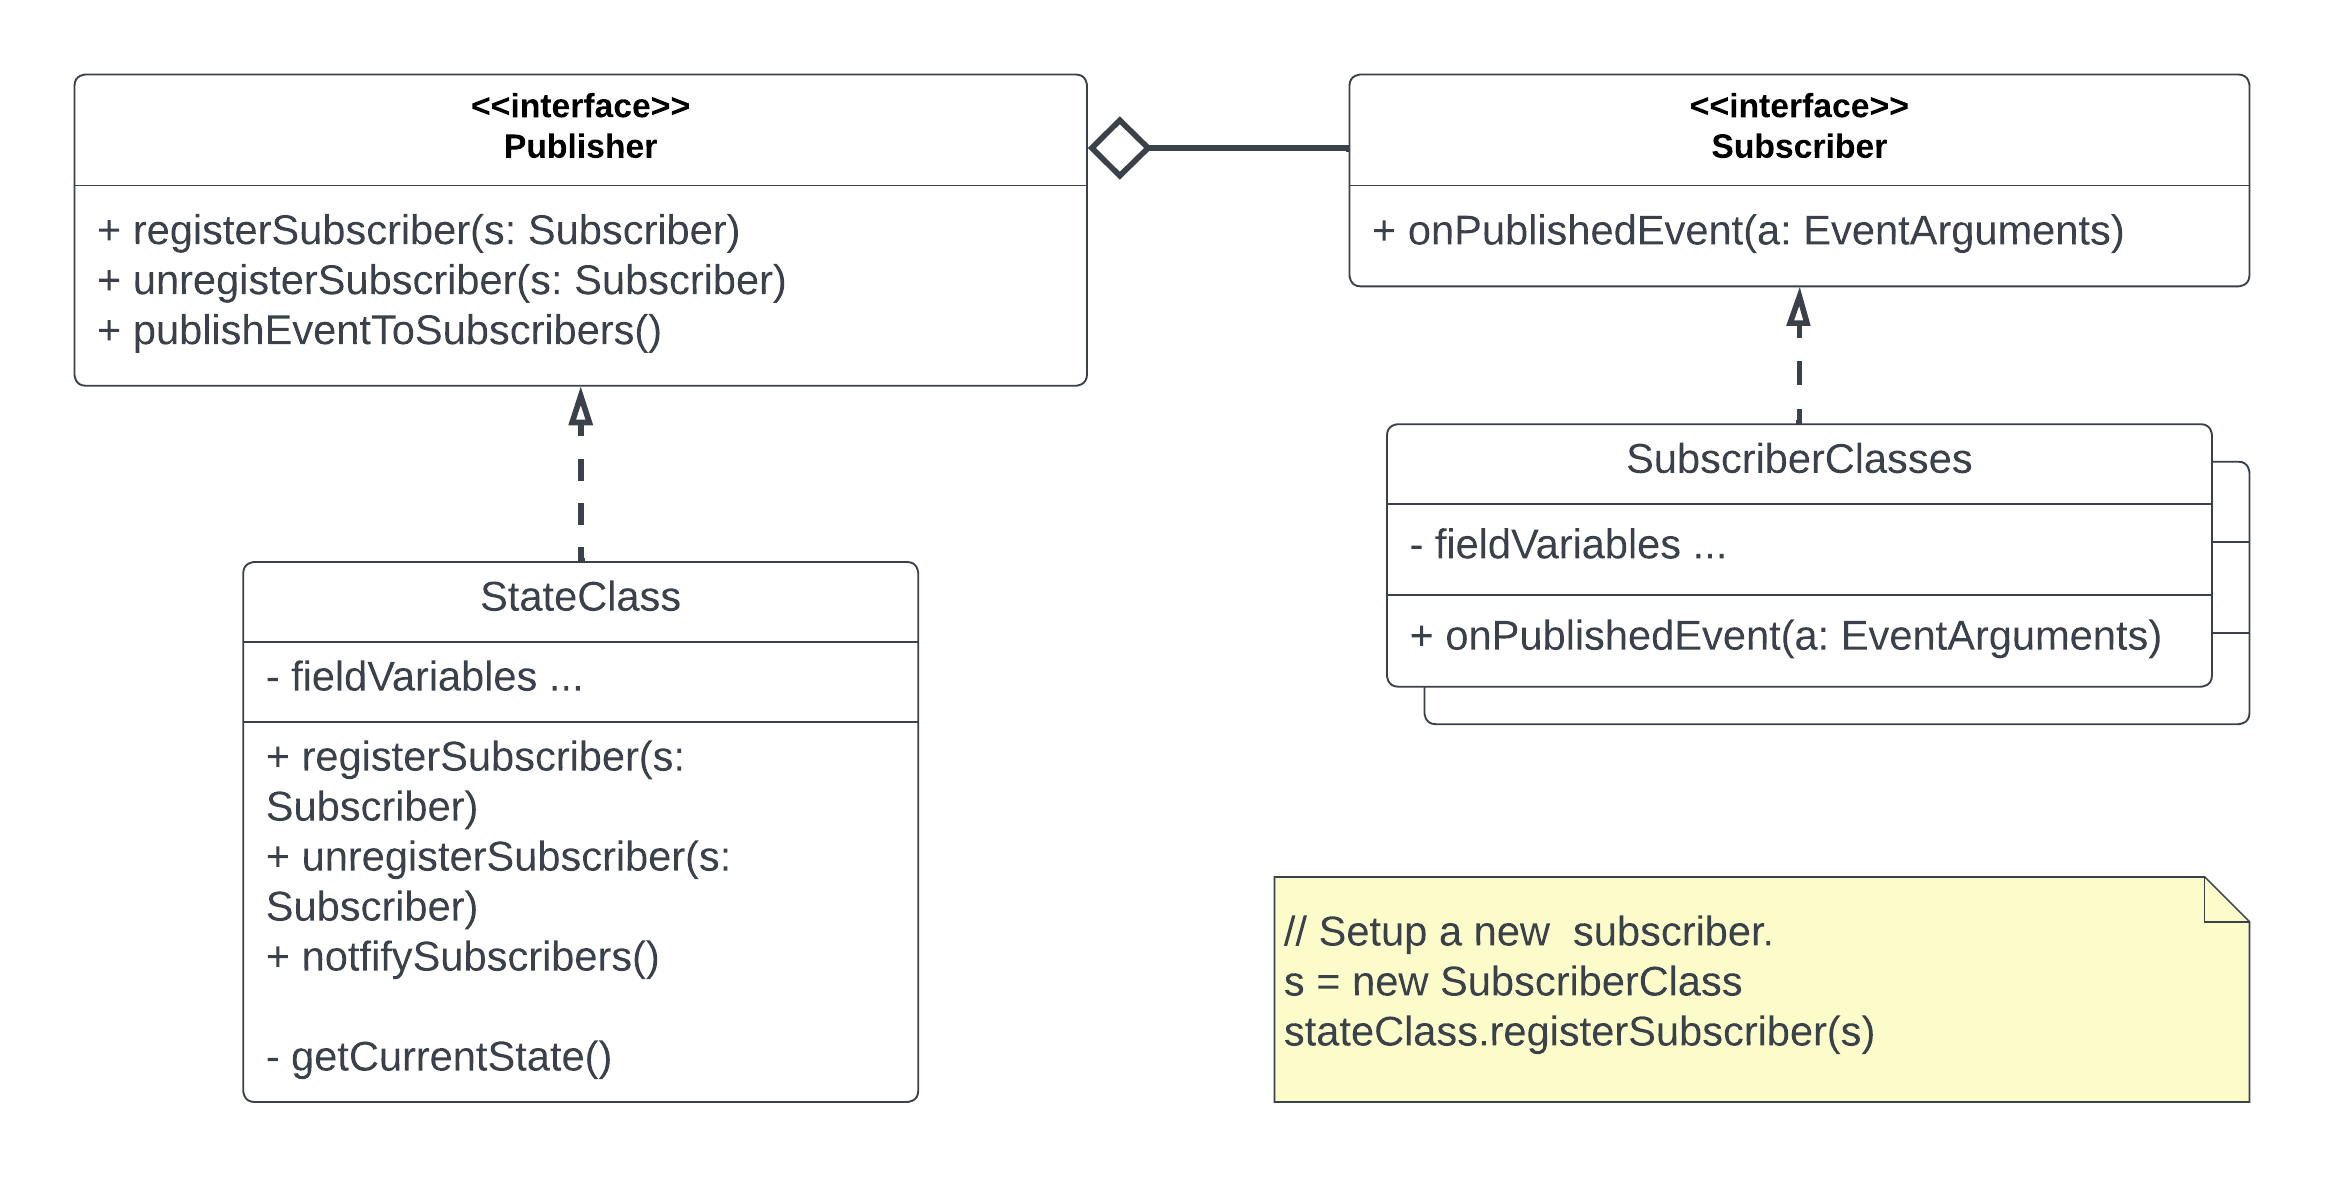
\includegraphics[scale=0.75]{Project_report/figures/theory/design_patterns/observer_uml.png}
      \caption{UML diagram of generic publisher/subscriber-relation implementation.}
      \label{fig:observer_uml}
    \end{figure}

\subsection{Overview of the Observer Pattern in Unity and C\#}
    Both the C\# programming language and the Unity API includes several features that facilitates the use of the Observer pattern. Most modern languages opt for a method-based implementation of the Observer Pattern, as compared to the class-based implementation as seen in figure \ref{fig:observer_uml}. The list that follows highlights some of the most prominent components that are used to promote the usage of this pattern:

\begin{itemize}
    \item \textbf{Delegates (C\#)}: Define a type representing a specific user-defined method signature, allowing for a method-based event system. This custom type can be realized with any method sharing the same signature as the delegate, enabling a type-safe way of passing methods as arguments. They resemble C++ function pointers but provide object-oriented capabilities by encompassing both a function and its associated object instance.
    
    \item \textbf{Event Handlers (C\#)}: Methods defined in the subscriber class that conform to a specific delegate signature, typically a delegate with two parameters: one object representing the publisher and one event data object containing event-specific information. These event handlers are responsible for processing incoming events and performing any necessary actions when the triggering event is published.
    
    \item \textbf{Events (C\#)}: A convenient feature in C\# built upon the foundation of delegates. They provide an easy way to define, subscribe, and publish events in C\#. Publishers define the event, while subscribers can subscribe or unsubscribe using the event handler. Events enforce encapsulation by allowing only the class that owns them to publish them while still enabling other classes to subscribe or unsubscribe at run-time.
    
    \item \textbf{UnityEvents (Unity)}: A built-in event class offering a flexible and powerful way to facilitate event-driven systems that can be configured in a user-friendly way through the Unity editor. Being serializable, they can easily be set up and managed through the editor using a drag-and-drop approach within the editor.
\end{itemize}

\subsection{Singleton}
    The Singleton pattern is a creational pattern that ensures only one instance of a specific class can be created at any given time, providing global access points to that instance. The pattern has garnered criticism for violating core object-oriented principles, such as The Single Responsibility Principle\footnote{The 'S' in SOLID. States that a class should only have one responsibility, promoting good separation of concern and modularity.}, promoting tight coupling, and making testing more difficult due to challenges in isolating tests, replacing instances with mocks, and managing shared global state. However, some argue for its responsible usage, applied only to classes that genuinely require a single instance and where global access is necessary. It is crucial to manage dependencies and shared states carefully to minimize the risk of creating hard-to-maintain, tightly-coupled code. Common use cases for the Singleton pattern in game development include managing access to different manager classes, such as managers for input, audio, or pooling.

    The pattern is implemented by having a private static field in the singleton class for storing the instance of the class. This instance is instantiated through a public static creation method, which uses "lazy initialization" to create a new singleton object instance through a private constructor if it is the first time the instance is being called, or returns the pre-existing instance otherwise. To ensure thread-safety in multi-threaded applications, a locking mechanism can be implemented to prevent multiple threads from creating separate instances simultaneously. This can be achieved using the "double-checked locking" pattern, where the lock is only acquired if the instance is null, reducing the performance overhead of locking in cases when the instance is already created.

    The pattern is implemented by having a private static field in the singleton class for storing the instance of the class. This instance is instantiated by having a public static creation method, that through "lazy initialization creates the new singleton object instance through a private constructor if it is the first time the instance is being called, and if not, simply returns the pre-existing instance. To ensure thread-safety in multi-threaded applications, a locking mechanism can be implemented to prevent multiple threads from creating separate instances simultaneously. This can be achieved by using the "double-checked locking" pattern, where the lock is only acquired if the instance is null, reducing the performance overhead of locking in cases when the instance is already created.

\subsection{State}
    The State pattern is a behavioral pattern that creates a modular and extensible system architecture for managing transition between different object states. The pattern does so by decoupling the logic for each possible state into a separate interface that a main class then manages by offering methods for interacting with different state objects and delegating any necessary command to the current state when told to. This main class can be described as mediator between different states, and offers the developers an user-friendly way of managing state actions and transitions.

    The pattern was first introduced by the aforementioned book "Design Patterns: Elements of Reusable Object-Oriented Software", and draws its inspiration from the concept of finite state machines (FSM) which are computational model used across a wide spectrum of domains such as control systems and artificial intelligence. A FSM consists of a finite amount of states, the initial state, and the adhering transitions between them. While both FSM and the State pattern deals with managing system behavior through various states and transition, FSM is a more general concept that focuses on the overall structure of a system, while the State pattern is a specific object-oriented concept focusing on adhering to good object-oriented principles.

    By seperating the state logic into a seperate interface, this makes it easy to accommodate for change and extensibility when modifying or adding a new state. This adheres to the Open/Closed principle\footnote{The 'O' in SOLID. Says that a class should be easy to extend without needing to modify any existing code.} as it allows developers to introduce new states without altering the existing state classes or the main class responsible for managing state transitions.

    The pattern is implemented by defining the common State interface, that should be able to handle any state specific requests and transitions. This interface is then realized by concrete states classes that provides their own unique logic and behaviour. To mediate between these states, you then implement a main class, sometimes called the Context class, that holds a reference to the current state and delegates function calls to it. This main class is also responsible for changing the current state based on transition logic defined in the concrete State classes.
    
    \begin{figure}[H]
      \centering
      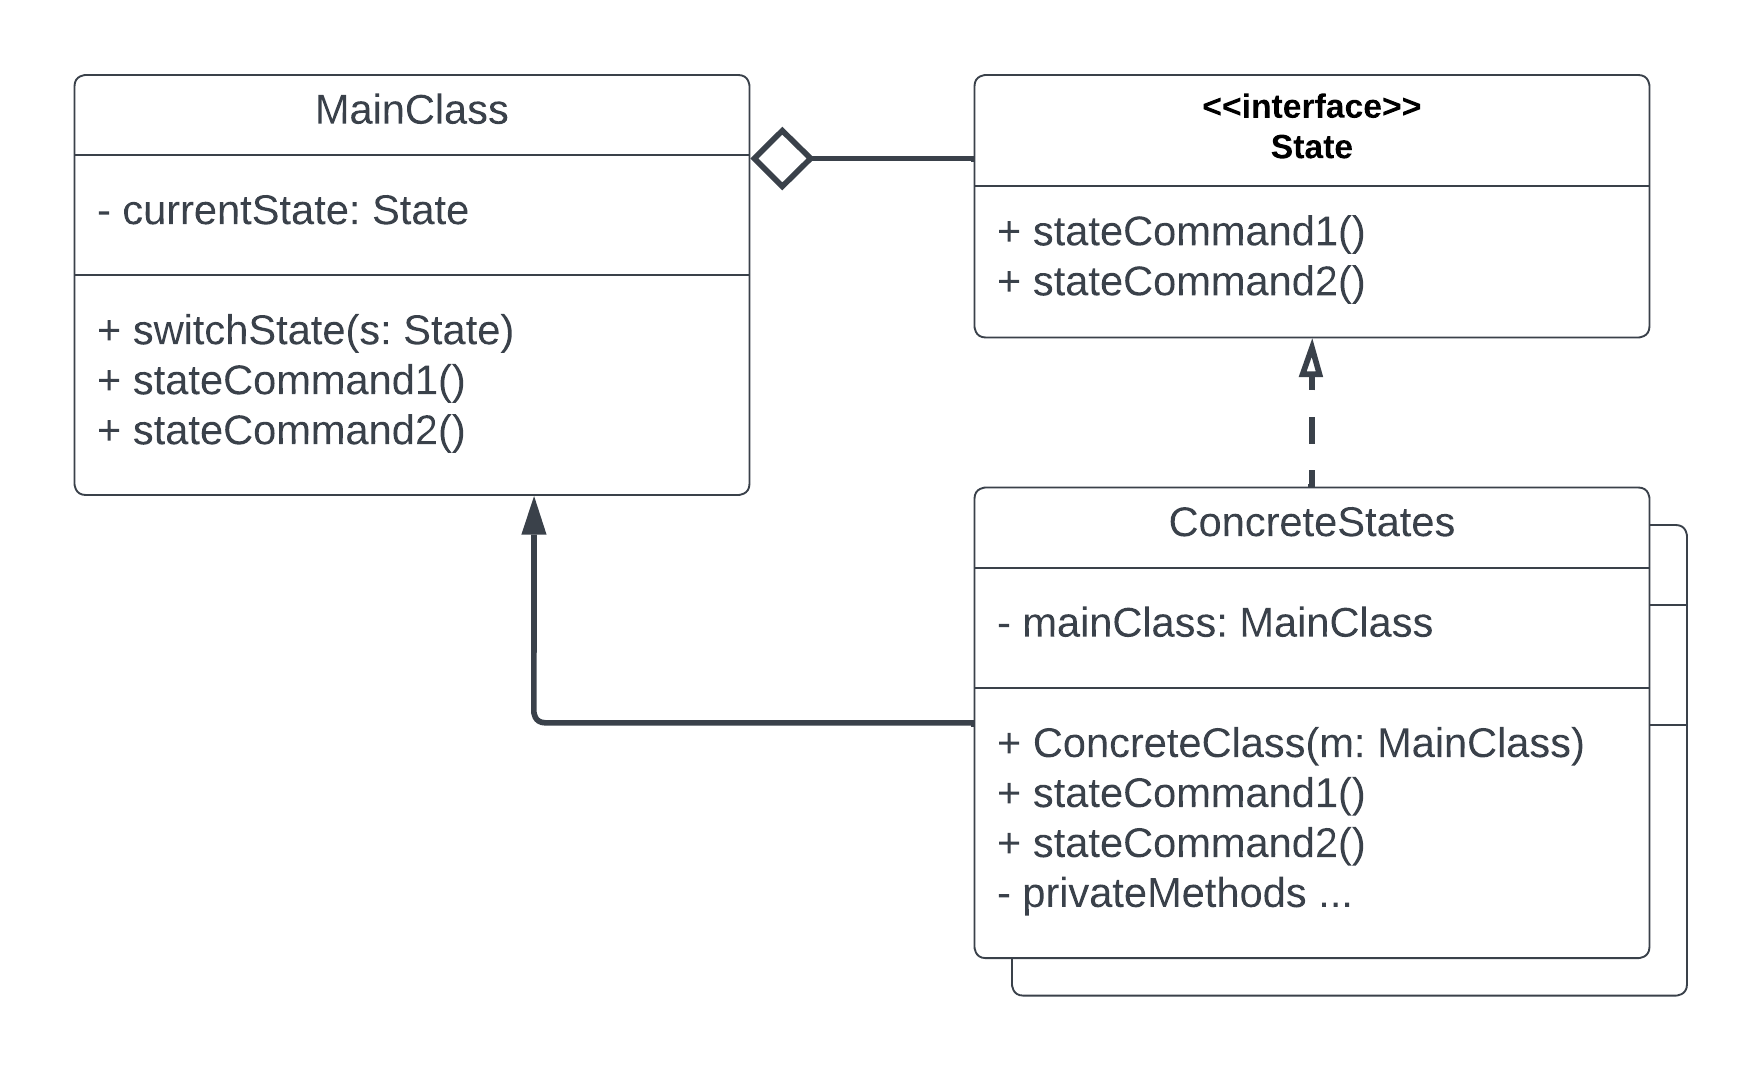
\includegraphics[scale=0.75]{Project_report/figures/theory/design_patterns/state_uml.png}
      \caption{UML diagram of generic State pattern implementation.}
      \label{fig:observer_uml}
    \end{figure}

    \vspace{50pt}
    \begin{itemize}
        \item https://www.amazon.com/-/dp/0195019199
        \item Design Patterns: Elements of Reusable Object-Oriented Software
        \item https://gameprogrammingpatterns.com/observer.html
    \end{itemize}




%% Hannes Kaulio
\section{OpenStreetMap}
    OpenStreetMap is a free database which contains geographical data. The database is maintained and updated by volunteers. Volunteers can collect data about geographical areas and add to the database for everyone to use. Data about features such as roads, railroads, buildings, trees, etc and their properties exist. 


% Methods
\chapter{Methods}
    % UPDATED BY MARCUS SCHAGERBERG, 2023
% CREATED BY WOLFGANG AHRENDT, 2021

\section{Tools}

% WRITTEN BY JAKOB WINDT, 2023
\subsection{Unity}

The traffic simulation tool is built in a well-known game-engine called Unity. There are a few reason why it was chosen as the development platform for the project instead of a similar game-engine like Unreal Engine. To begin with, C\# is the main programming language supported by Unity, which some of the team members had previous experience with. Furthermore, C\# is a higher level language compared to C++, the main language of Unreal Engine, making it easier for the team members without experience to learn. Because of this, the time it took to begin programming in the early stages of the project was most likely shorter, compared to if Unreal Engine was chosen as the platform.
\\\\
Another reason would be that Unity comes with the Unity Asset Store, a marketplace for acquiring creator made assets. This feature is important because, for example, instead of having to create custom models for the vehicles, they could instead be purchased using the given budget. This saves a lot of time, that could be better spent on other parts of the project. One of the more notable purchased assets is Edy's Vehicle Physics that are used to rig vehicle models with realistic physics. Instead of having to develop custom vehicle physics for each model, the team could instead use the asset to quickly configure a model with physics.
\\\\
The final reason why Unity was chosen, is because of its flexible developing structure. The level of customization available inside the engine is a lot greater when comparing to Unreal Engine. However, because of this, Unity ends up being more unstable whereas Unreal is far more stable and robust. 

% WRITTEN BY JAKOB WINDT, 2023
\subsection{GitHub}

A commonly used tool when developing software in larger groups is Git. Git is a free and open-source version control system that allows its users to collaborate in a efficient and easy way. 
\\\\
GitHub is an online software development platform that utilizes Git to store and track software projects. It allows for users to work in their own separate branches, and later merge those into the main repository. Before a team member could merge their new code to the main repository, the code would have to be reviewed by at least one other team member to ensure that the code was well commented, functional, and that it follow the C\# coding standard.

% WRITTEN BY JAKOB WINDT, 2023
\subsection{Trello}

It was decided early on that the projects work flow should follow the SCRUM and Agile software development practices. Trello is a website that hosts scrum-boards in an user-friendly way. This allowed the team to keep track of what needs to be worked on in the project during the sprints. A sprint is a set time period when new tickets are made, and completed.

% WRITTEN BY JAKOB WINDT, 2023
\subsection{Balsamiq Wireframes}

During the first stage of creating a UI, its important to start with a simple mock-up design. This is what the tool, Balsamiq Wireframes, is used for. The user can quickly design wire frames depicting how the UI will appear during different times in the program. This includes everything from buttons to pop-up menu's that might appear in the simulation tool.

%% WRITTEN BY JAKOB WINDT, 2023
\subsection{Third-Party Assets}

Built into Unity is their asset store. Instead of creating everything from scratch, the team opted to purchase some assets. An asset can be anything from a 3D model to animation and scripts. The two main assets purchased for the project are Edy's Vehicle Physics and European Road Signs. Edy's Vehicle Physics is a package that includes a tool that allows its user to easily implement realistic vehicle physics into 3d models. This saves a substantial amount of time in the end because there would be no need to create custom physics attribute for each vehicle model. 
\\\\
As the name states, the European Road Signs assets include a plethora of street signs, as well as an editor to customize them. Without this asset, there would have been a need to create custom 3D models and texture, which no team member had previous experience with.

\section{Simulation Design and Implementation}

\subsection{ABM}

% WRITTEN BY HANNES KAULIO, 2023
\subsection{Road Generation}
In order to achieve realistic roads with adequate curves, composite Bézier curves were used. The Bézier control points will shape the road and its characteristics. A number of parameter can be changed in the Bézier path to change the appearance. The position and sharpness of the turn can be modified by changing were the control points are placed in relation to each other. 
\inlineimage{figures/method/road_generation/bezier_path_unity.png}{Composite Bézier path }{0.5}

While the Bézier curves give a good ground level for the road implementation, it is hard to implement and build logic based on it since it is a continuous path. The Bézier logic and its control points was abstracted away with a node implementation placed on top of the Bézier path. A number of nodes called RoadNodes is placed along the Bézier path at a rate dependent on curve of the road. The nodes are all connected the its previous and its next node along the path. The goal of these nodes is to carry enough information to procedurally  build the physical road as well as carry the logic needed for agents to navigate the environment.
\inlineimage{figures/method/road_generation/roadnodes.png}{Visual representation of RoadNodes places along a Composite Bézier path}{0.5}

By using the RoadNodes, generating the road mesh is possible. The mesh is precedurally generated by placing verices 
        
\subsection{Intersection Generation}

\subsection{City Generation}

% WRITTEN BY HANNES KAULIO, 2023
\subsection{Navigation}
The basic navigational responsibility of each agent is the ability to follow the road lanes, avoid colliding into other agents, follow the traffic rules and being able to navigate to a given position.
\\\\
In order to achieve a lane following agent, a navigation path is created for each road lane. The path is created as a double linked list. The nodes are insert along the lanes Bézier curve at a constant rate. Each node in the linked list store all information needed to navigate that lane. The position of the node, the agent that is currently on the node and special traffic rules the vehicles need to follow are stored on the node. Traffic signs such as stop sign are represented as a node and the traffic logic can be accessed by the agent when they encounter the node. 
\\\\
The agents steer towards a node that is a certain distance in front of the car. This distance is influenced by the current speed. By steering towards nodes that are in front of the agent, a smooth and reliable steering is achieved. Similarly to steering, breaking is accomplished by looking at nodes at a certain distance ahead. When a node with stop logic is found, the agent will break and stop before that node. This is done by looking for stop nodes at a distance ahead equal to the break distance of the agent. The agents also claim each node they are over so other agents can stop when the node at the break distance is claimed.                                                
\\\\

To enable the ability to navigate the roads, a weighted directed graph is created from the roads.
The graph nodes are all the road endpoints and intersections. The edges between the nodes are weighted with a cost that is calculated as the distance * the speed limit.
The agents navigate to a given end node by receiving a path of edges from the A* algorithm. When an agent drives up to a intersection, the intersections give a new road path to follow given the navigation node the agent is traveling to.

\section{Performance}

\subsection{Quality vs Performance}

\subsection{Performance Benchmarks}


\section{Graphics}

\subsection{Animations}

\subsection{Environment Materials and Textures}


\section{User Interface}

\subsection{Statistics}

\subsection{Design}

% WRITTEN BY MARTIN BLOM, 2023
\section{Work flow}
When developing any software larger than just a single use script, the amount of work and information can quickly grow beyond the level of ones own simultaneous comprehension. Therefore these kinds of projects require rigorous planning and strategizing to not get lost in all the different tasks and do them in a smooth and reasonable order, that allows for parallel continuous progress.
\\\\
To achieve this a strict work flow framework was developed, where the first step was to analyze the work load and disposable time. This included drafting a time plan for the whole time scope of the project \ref{fig:time-plan}. 

\begin{figure}[H]
    \centering
    \fbox{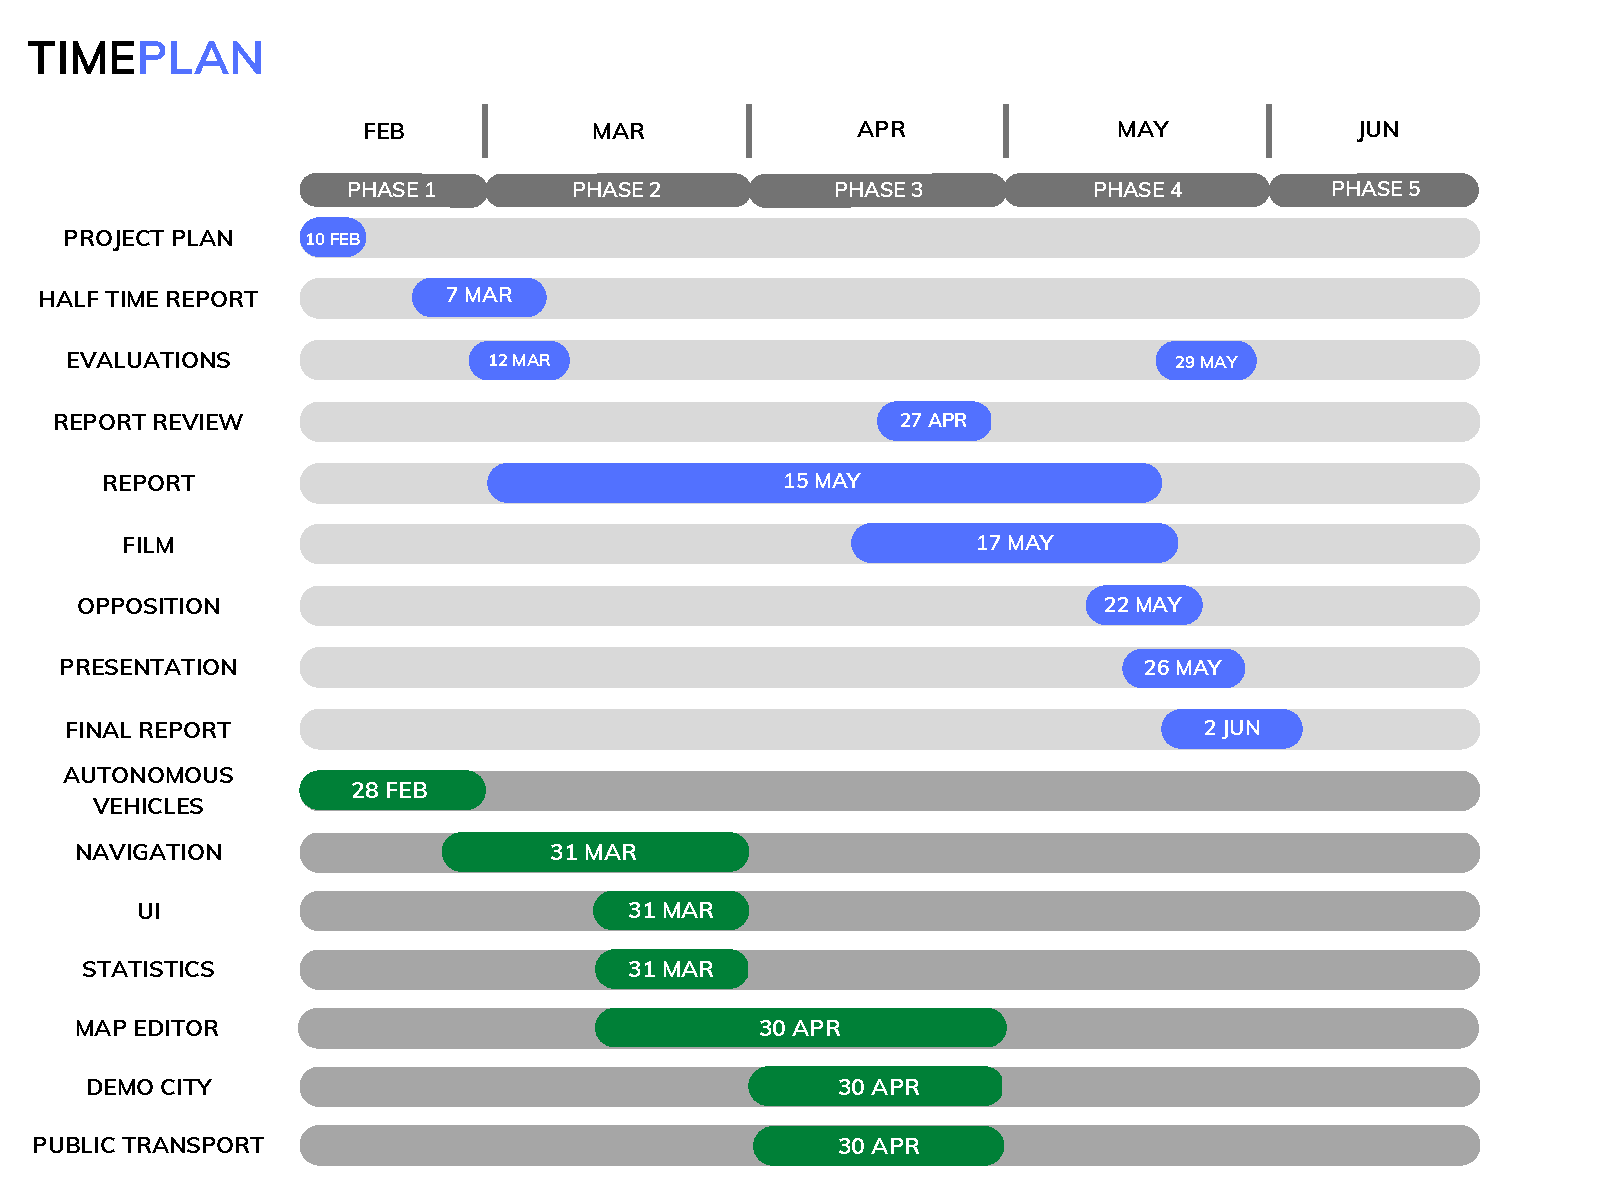
\includegraphics[scale=0.5]{Project_report/appendix/Time_plan.pdf}}
    \caption{Project Time Plan}
    \label{fig:time-plan}
\end{figure}

With this it's now much easier to keep track of the general progress of the project, as well as helping with planning short term goals. Coincidentally this is the next step of the work flow model. The short term goals where planned using a scrum framework with weekly sprints, explained in \ref{sub:weekly-sprints}. These sprints were upheld for the duration of the project to keep a stead flow of progress, together with the time plan they create a very clear way of seeing the current state of completeness. 
\\\\
The third aspect of the work flow is the approval of progress. As mentioned earlier a large project requires a substantial amount of planning to not get lost. The approval of progress can be seen as just as important as the planning and execution itself. Without a popper method of approving new advancements/functionality, the project can quickly falter. If progress never goes through the process of approval many things can go wrong. Evidently, badly written code can cause issues that are easily preventable with a quick inspection. Code can even be considered good but with no input from the rest of the team, visions of how higher order elements will be implemented can differ. This can implicitly create  more complex problems much further on, which can be very hard and time consuming to resolve. To solve this, code review's \ref{sub:code-reviewing} for every change made are part of the work flow.  

\subsection{Weekly Sprints} \label{sub:weekly-sprints}
The weekly sprint model stems from the scrum framework, which is a framework for developing and sustaining complex products. The sprint model follows 4 repeating stages of development: Planning, Implementation, Review and Retrospect.
\\\\
Each sprint starts out in the planning stage, where a meeting is held to set up this sprints goals. This includes moving/creating stories for the backlog as well as the current sprint. The stories are mainly chosen by the project manager then developed in unison with the scrum master and input from the rest of the team.
\\\\
The next stage of the sprint is the implementation itself. This is the time were the teams focus is solely on delivering good quality solutions to complete all of the current sprints stories, and eventually working on the backlog as time is presented.
\\\\
Next up is the review stage, not to be confused with code reviewing \ref{sub:code-reviewing}. In this stage another meeting is held called a "Demo meeting", where all members get to do a small demonstration of all their progress during the sprint. This is an important step to onboard all members on new functionality and make sure that desired behaviour is achieved. When a story is regarded as fully complete it's archived to make room for new ones.
\\\\
Lastly the retrospect stage, which is usually carried out following the review stage. In the retrospect stage the current sprints efficiency and quality is discussed. And plans/ways to increase these and the overall effectiveness are considered. When all is done the cycle begins anew until the project is done.

\subsection{Code Reviewing} \label{sub:code-reviewing}
% TODO 
% describe code review process

\section{Testing}

% Results
\chapter{Results}
    % UPDATED BY MARCUS SCHAGERBERG, 2023
% CREATED BY WOLFGANG AHRENDT, 2021
% WRITTEN BY JAKOB WINDT, 2023

This section will give an account for different results gathered from both our experience with the product, performance benchmarks, and feedback that were collected during user testing. 

\section{Final product}
    The end product is a simulation tool that is capable of simulating vehicles driving in a road network. The road network can either be generated through an imported OSM file, or custom built with the use of the built in Unity Editor. The road network has support for both three and four way intersections. These intersections can either be controlled by traffic lights or stop signs depending on the user's needs. The vehicles themselves are all capable of individually navigating a correctly built road network. The vehicles interacts with their surroundings using the RoadNodes and LaneNodes built into the roads. From these nodes, the vehicle can collect data about whether a node ahead of them is occupied as well as the current speed limit of the road, and if the vehicle needs to brake.

    To use the simulation tool, the users can interact with the simulation through the provided UI. It consists of a main menu, with an included settings page. In addition, there is an overlay menu, that is visible while the simulation is running. With this overlay menu the user can access statistics about an individual vehicle or the entire road network. The statistics are represented through a series of data points and graphs to easily display different statistical aspects of the simulated road network. The user can also change the number of simulated vehicles.

    By using the Unity Editor, the user can as mentioned customize the simulation world. The user can also create roads, add intersections, and add POIs. Furthermore, it is possible to add buses that travel along the bus stops. Parking lots can also be added. These parking lots can either be attached to a road as a street side parking, or as a separate parking lot.

\section{Performance} \label{performance-benchmark}
    % Mention that it was found through the profiler that one of the heaviest operations is updating the vehicle physics
    To test the performance of the tool, an automated testing utility described in section \ref{performance-method} was used. The tests were run on a simulation of the road system for Masthugget, a district of Gothenburg. The tests were run both in the quality mode as well as the performance mode. The test results are compiled in Table \ref{Tab:performance-benchmark-results}.

\begin{table}[ht]
    \caption{Performance test results}
    \centering
    \begin{tabular}{|c|c|c|}
        %% ----- >>> FIRST ROW -----
        \hline
        \multicolumn{1}{|c|}{Configuration} 
        &
        \multicolumn{2}{|c|}{Result}
        \\\hline
        %% ----- <<< FIRST ROW -----
        %% ----- >>> HEADERS -----
        Number of vehicles & Quality FPS & Performance FPS
        \\\hline
        %% ----- <<< HEADERS -----
        %% ----- >>> VALUES -----
        
        5 & 192 & 205
        \\\hline
        50 & 191 & 203
        \\\hline
        100 & 189 & 203
        \\\hline
        250 & 71 & 102
        \\\hline
        500 & 30 & 48
        \\\hline
        1000 & 10 & 25
        
        %% ----- <<< VALUES -----
        \\\hline
    \end{tabular}
    \label{Tab:performance-benchmark-results}
\end{table}

% WRITTEN BY FELIX JÖNSSON, 2023
\section{User tests}
    User testing in software development is an important aspect of a successful end product. It gives the developers insights into how their software is actually perceived in a deployed environment, and how their intended audience interacts with it. This section presents an account of our performed user testing and the feedback received. The testing was conducted with two distinct groups: "experienced testers", and "generic testers". 
    
    % WRITTEN BY MARCUS SCHAGERBERG, 2023
    \subsection{Experienced Tester}
        The first test subject had prior experience in a transportation planning software called PTV Visum, which is the world's most popular software of its kind when it comes to aiding strategic and operative decisions\cite{visum}. Compared to Visum which is set in 2D, the user felt that our tool provided more context, and that it was easier to understand the road network. The test subject pointed out that it was harder to see the road connections and intersections in PTV Visum. However, Visum offered a better view for larger networks. The user appreciated the simulation of individual vehicles compared to Visum, which displays traffic as a value of the number of vehicles per road, and felt that it improved the intuition for smaller networks. Being able to see statistics related to individual vehicles was also pointed out as useful. The test subject felt our tool lacked some customisability that Visum offers, where you can change parameters such as road capacity that affect the simulation. The user mentioned that Visum had a learning curve to understand the buttons and features, which was easier to do in our tool although it does not offer as granular control over the traffic as Visum does. The test subject was not able to use the public transportation feature as it was not done at the time of testing, but expressed interest in it and thought that it was a great idea that Visum lacked. Colour coding the roads based on the congestion level was being implemented at the time of testing, and was something the subject mentioned would also be helpful.

        The tester felt that our tool was easy to understand, and significantly simpler to use for presentation purposes than Visum, which was said to be more technical and harder to understand at first glance. The user had used Visum to demonstrate their solution, and said that it was difficult to find a good way of visualising and presenting it. 
        
        %%It was also thought that our tool would be useful for education purposes, and that it would fit well for teaching different concepts in transportation planning, as it is intuitive and easy to understand what is happening in the simulation.

        Apart from the functionality compared to Visum, the test subject also had feedback regarding the UI. The user thought that it was confusing that there were separate buttons for the statistics, depending on if it was showing individual statistics for a vehicle or aggregated statistics for the entire road network. It was also expressed that it would be easier to navigate using the mouse for adjusting the camera rotation while keeping the keyboard for moving the camera around, and that it felt slow to move around a larger network.
    % WRITTEN BY FELIX JÖNSSON, 2023
    \subsection{Generic Tester}
    The project also conducted user testing on a group we have classified as "generic testers". These individuals possessed no prior experience with any form of simulation software, and the primary objective during these tests was to discern potential deficiencies in the UX design. Some feedback that was acquired included the lack of alternative control schemes. Every tester tried to move around the simulation using the arrow keys, though the tool's movement keys are WASD. Once identified, the camera movement felt good, but they would have liked a clearer communication of the control scheme somehow. This confusion regarding the control scheme also extended to how the user moved between cameras, and some users felt that it was hard to tell the difference between the follow camera and default camera depending on your initial zoom when transitioning to the default camera.

    Furthermore, all generic testers reported a preference for more prominent signaling of the various UI functionalities. This could potentially be achieved through the introduction of informative tooltips, the strategic use of intuitive visual icons, and the implementation of an initial user onboarding walkthrough, that succinctly explains each feature. For example, one tester reported that they felt unsure if they had actually managed to spawn any vehicles when they had pressed the "spawn vehicle"-button, and would have liked some feedback on their input or an explanation of how the spawning functionality actually worked.

% Conclusion
\chapter{Conclusion}
    % WRITTEN BY JAKOB WINDT, 2023
This section will summarize the project. It goes into detail on how future problem presentations might arise, and how the tool might be configured to be used in other fields. Lastly, it will quickly summarize some of the skills that were learned during the project.

    % WRITTEN BY MARCUS SCHAGERBERG, 2023
    \section{Distinction from other tools}
        There are a few key points differentiating this tool from most others. Firstly, it is the focus on accessibility, allowing a much wider audience to use the tool compared to most existing solutions that are focused around civil engineer usage. One advantage of this is that it enables regular citizens to effectively give their own input and suggestions for improvements in their city.

        Since the purpose of the project was to develop an accessible traffic simulation tool, the input from the user testing sessions was vital in order to confirm that this was achieved. Through the combination of a tester with prior experience and training in an existing tool and the generic testers that gave valuable feedback regarding the user-friendliness, it was clear that the tool was accessible and easy to use. Constructive feedback was also provided, which was used to improve the tool. An important part of this, as well as a distinction from most other tools, is the 3D environment instead of the more widely used 2D alternative. This makes it harder to understand large road systems, but was identified to be an improvement for smaller networks as well as making the tool more accessible according to the testers.

    % WRITTEN BY MARTIN BLOM, 2023
    \section{Additional Knowledge}
        There are two main areas where additional knowledge would have had the most impact on the final product. The first area revolves around programming, and the game engine that was used. To start off, a large portion of the group members had never worked on a project of this size, nor in a team this big. With a lack of experience, we quickly found it hard to keep progress organized which resulted in the repository becoming cluttered. With more experience and prior knowledge in working with larger software projects, the workflow would have been smoother, and mistakes could have been avoided.

        The other area where more knowledge would have been beneficial, is surrounding infrastructure engineering, traffic flow modeling and ABM systems. With some background in these subjects, it would allow for increased accuracy and quicker development of the vehicle simulation system. Moreover, it would have given us a better understanding on which statistics are most important, and the best way to present them to the user.

    % WRITTEN BY MARCUS SCHAGERBERG, 2023
    \section{Future Problem Presentations}
        Given the insights gained throughout the development process, another area that might benefit from a tool like this would be airports. They, like the road networks, have traffic they need to handle, and require planning to construct airports with large capacities. They have taxiways where the airplanes move between the gates and the landing strip. These relocating planes interfere with other planes trying to take off or land, which means that a good traffic flow is a requirement for a well-functioning large scale airport. A simulation tool like this one could be tailored towards airports, investigating the different synergies that affect the performance of an airport. The tool should also allow for different airport configurations to be simulated in order to evaluate them. Airport traffic brings with it a different set of challenges and relationships. One example is that all airport traffic is scheduled, which means that well planned arrival and departure times can improve the performance, increase the capacity and the overall throughput of an airport.

        As the future looks to bring more and more autonomous vehicles, transportation planning tools could play an even more important role. If all vehicles are autonomous, the traffic could be centrally controlled to avoid congestions, and balance the load in the road system to optimise its performance. A tool like this could be extended or repurposed in order to analyse these future traffic flows. New possibilities also emerge, since solutions could be based around the fact that the traffic is autonomous, and can therefore easily be redirected to better utilise the available road network. Perhaps it would be beneficial to redirect some vehicles on slight detours, making the travel time slightly longer. This could ease the traffic in some areas, and better distribute the traffic, to overall decrease the travel times in the road system as a whole.


    % WRITTEN BY JAKOB WINDT, 2023
    \section{Future Usage of the Simulation}
        In the future, many new use cases can be developed for the current simulation. An example for this could be to convert the simulation to a video game, allowing users to select a real-life location, and then drive around in that location with realistic traffic. Other than the previously mentioned improvements, the only feature that would have to be implemented is a way for a user to drive a vehicle on the road. This could quickly be implemented due to Unity's vast support for user inputs and camera control.

        Similarly, the simulation could be converted to a tool that would help people learn how to drive. In the same way, first person controls and cameras could be added, which could allow the user to use driving simulator hardware such as a steering wheel, pedals, and a gear shifter. This could be beneficial to driving schools since it could assist the students during the early stages of learning how to drive a car. The student would learn the basics in the simulator, without the risk or cost that comes with driving a real car in traffic with vehicles.
    
    % WRITTEN BY JAKOB WINDT, 2023
    \section{Learning Outcome}
        If we were to redo the project from scratch, we would have changed a few aspects of our approach. To begin, we would have lowered the scope of the project, so that we instead could focus on improving the quality. This would result in a simulation with fewer use cases, but with better core functionality. Therefore allowing the project to grow exponentially with more features in the long term, due to the added stability. Another aspect that would change, is that our custom road generator tool would be prioritized to be implemented. With access to this asset from the beginning, we could instead spend our time focusing on adding new features, and improving the simulation at its core.

        In the end, this project resulted in us learning numerous new skills which would further our expertise as we continue to grow and learn. In the beginning of the project, only a few of us had used Unity before, and only to a limited state. Now, we are all knowledgeable within the game development platform. In a similar way, this is reflected in many parts of the project, including but not limited to; Git, the scrum framework, C\#, road network design, and more importantly, working efficiently as a software development team.


% References
\cleardoublepage
\addcontentsline{toc}{chapter}{Bibliography}
\bibliographystyle{IEEEtran}
\bibliography{bibliography}

% Appendix
\cleardoublepage
\begin{appendices}
    \setcounter{page}{1}
    % Capitalized roman numbering starting from I (one)
    \pagenumbering{Roman}
    \chapter{Appendix 1}
        This is where we will place appendix 1
    
    \chapter{Appendix 2}
        This is where we will place appendix 2
\end{appendices}
\end{document}